\chapter{Desarrollo}
En este capítulo se presenta el método empleado para preprocesar los mamogramas
digitales.

\shorthandoff{>} 
    \input{flowcharthoriz.tex}
\shorthandon{>} 

\section{Etapa de recolección}
Las mamografías originalmente almacenadas en discos compactos, fueron extraídas
y ... , removimos los datos privados de las imágenes, los únicos campos son los
que se muestran en la \ref{table:dicomtags} 

\begin{table}[h]
  \caption{Etiquetas DICOM que permanecen en la imagen} 
  \label{table:dicomtags}
\begin{center}
{\small
    \begin{tabular}{c|c}
    \hline

    {\bf Etiquetas} & 
    {\bf Descripción} \\
    \hline
           (0000, 0001) & Bits alojados \\
           (0000, 0001) & Bits alojados \\
           (0000, 0001) & Bits alojados \\
           (0000, 0001) & Bits alojados \\
    \hline
    \end{tabular}
}
\end{center}
\end{table}

%Las tareas de \textit{scripting} se llevaron a cabo con el lenguaje de
%programación Python y la libreria PyDICOM.

\section{Método}
En esta sección se describe el método empleado para preprocesar las imágenes.

\subsection{Reducción del área de trabajo}
Los mamogramas recolectados tienen un -fondo- negro que cubre gran parte de la
imagen. Con el fin de acelerar el tiempo de ejecución de los algoritmos es
necesario remover esa área.

\subsection{Conversión de bits}
Las mamografías que se obtuvieron son de 12 bits. Sin embargo al visualizarlas
se obtiene una imagen opaca, esto es porque ...

\subsection{Eliminación de ruido}
Se elimina el ruido.

\subsection{Mejora del contraste}
Se mejora el contraste.

\subsection{Compresión} \label{compression}

%This is the final phase in our method. It deals with image compression. A
%compressed image takes less time for transmission, processing, and less storage
%capacity. We applied a technique introduced by AbuBaker
%\cite{abubaker2006mammogram}  abubaker2007efficient}. It aims at compressing an
%image with minimal loss of quality. 
%
%%We introduced small changes to the original method, making the bit conversion
%%with the algorithm proposed for the enhancement and applying after that a
%%normalization step.
%
%The applied method consists of three steps: image shrinking procedure, pixel
%depth conversion, and image enhancement. Description of each step follows. 
%
%\subsubsection{Image shrinking procedure.} 
%Here, we will find the maximum shrinking level of the image. It takes three
%substeps:
%
%\begin{enumerate}[a)]
%    \item Obtain the image histogram (see Fig. \ref{comp:a} and \ref{comp:b}). %% DESCRIBIR QUE SE HIZO AQUI
%    \item Modify the histogram by deleting the unused gray levels (gaps) in the
%    histogram. The result will be a right-skewed histogram, as shown in Fig.
%    \ref{comp:c}.  
%    \item Generate an image based on the new histogram. The new image will be
%    quite dark due to the gray levels being located in the dark side section, Fig. \ref{comp:d}.
%\end{enumerate}
%
%\begin{figure}[h]
%  \begin{center}
%    \hspace{\fill}
%    \subfloat[\label{comp:a}]{\includegraphics[height=30mm]{images/original-mammogram-16bits}}
%    \hfill
%    \subfloat[\label{comp:b}]{\includegraphics[height=30mm]{images/original-image-histogram}}
%    \hfill
%    \subfloat[\label{comp:c}]{\includegraphics[height=30mm]{images/shrunk-histogram}}
%    \hfill
%    \subfloat[\label{comp:d}]{\includegraphics[height=30mm]{images/dark-mammogram}}
%    \hspace{\fill}
%  \end{center}
%
%  \caption{Shrinking procedure. \subref{comp:a} original mammogram,
%  \subref{comp:b} histogram of \subref{comp:a}, \subref{comp:c} histogram shown
%  in \subref{comp:b} after being shrunk, and \subref{comp:d} is the dark image
%  generated from the shrunk histogram.} 
%  
%  \label{img:shrinking-one} \end{figure}
%
%%\begin{verbatim}
%
%%\end{verbatim}
%
%\subsubsection{Pixel depth conversion.} 
%In this step the goal is to reduce the size of the image. Three substeps are
%involved:
%
%\begin{enumerate}[a)] %% NECESITAMOS AGREGAR DESCRIPCION DE CADA UNO DE ESTOS SUBSTEPS
%    \item Extract the histogram of the shrunk image.
%    \item Find the maximum shrinking level for the image.
%    \item Reduce image from 16 to 8 bits. 
%\end{enumerate}
%
%The shape of the original histogram shown in Fig. \ref{comp:b} is quite similar
%to the histogram of the resultant image shown in Fig. \ref{comp:g}. Peaks look
%the same, which indicates that the concentration of gray levels remains
%unchanged.
%
%\begin{figure}[h]
%  \begin{center}
%    \hspace{\fill}
%    \subfloat[\label{comp:e}]{\includegraphics[height=30mm]{images/dark-mammogram-histogram}}
%    \hfill
%    \subfloat[\label{comp:f}]{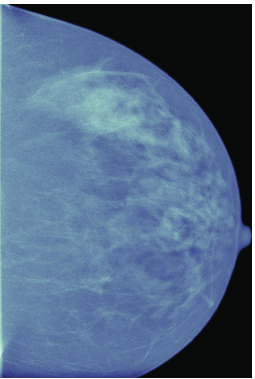
\includegraphics[height=30mm]{images/compressed-mammogram-8bits}}
%    \hfill
%    \subfloat[\label{comp:g}]{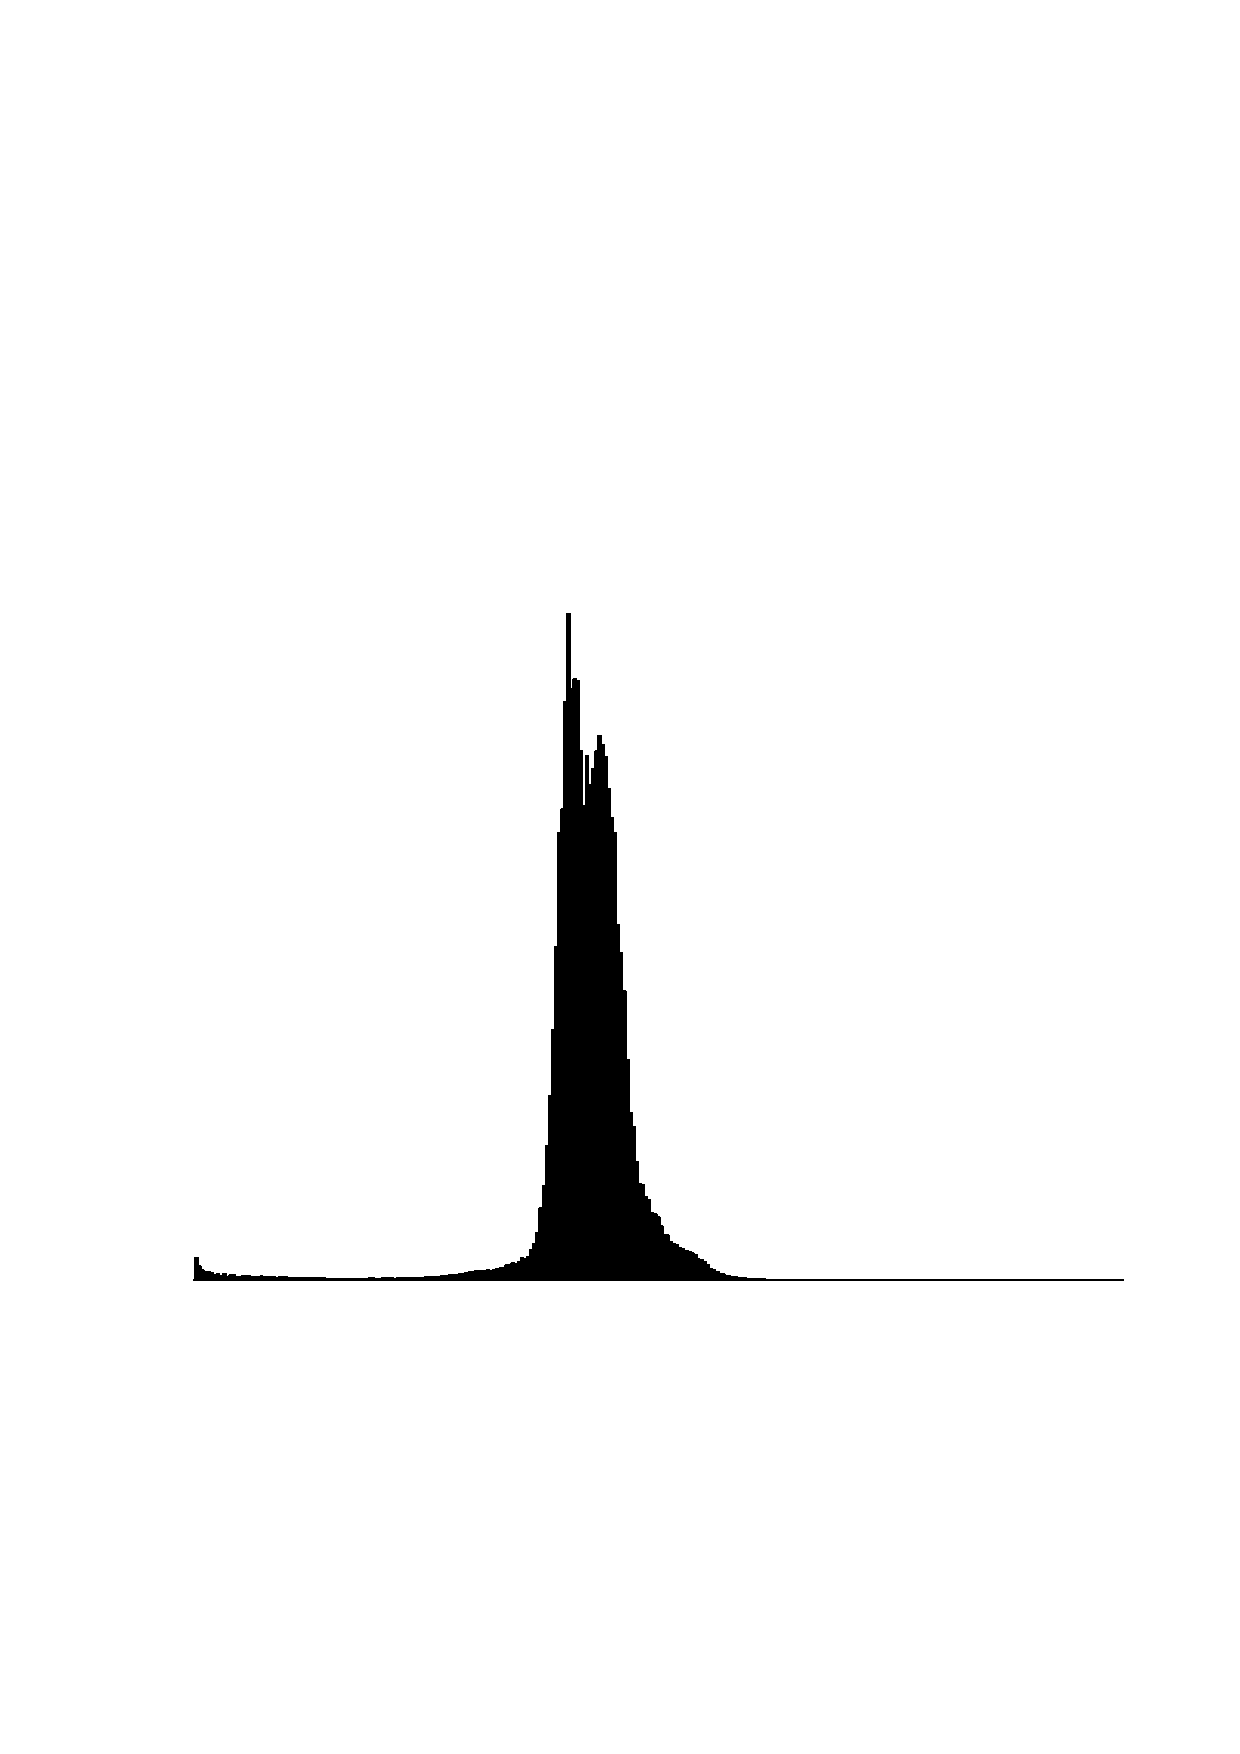
\includegraphics[height=30mm]{images/compressed-mammogram-histogram}}
%    \hspace{\fill}
%  \end{center}
%
%  \caption{(a) shows histogram generated from the dark mammogram, (b) is the 8 
%  bits mammogram, and (c) is the histogram of 8-bit image, which is similar to 
%  the original mammogram.} 
%  
%  \label{img:shrinking-two}
%\end{figure}
%
%\subsubsection{Enhancing pixel depth conversion.}
%This step aims at improving brightness of the image obtained from pixel depth
%conversion.  Afterwards, image conversion from 16 to 8 bits using an efficient
%coefficient takes place.  Medical information carried by the image should be
%maintained. %% AGREGAR REFERENCIA A UNA FIG., SI LA HAY

% change the words in this paragrap

%This final step is useful like a normalization process. Below is presented the 
%Matlab code used:

\definecolor{bg}{rgb}{0.9,0.9,0.9}
\begin{minted}[linenos=true, 
               %fontfamily=fi4, 
               fontseries=ubx,
               bgcolor=bg, frame=lines]{matlab}
% Get the size of the image
% Based on Abubaker code
[height width] = size(image);
imageCopy = repmat(uint8(0), height, width);
divider = 0.0;
maxLevel = double(usedGrayLevels);

while 1
    divider = divider + 0.01;
    if maxLevel/divider <= 255
        break;
    end
end
fprintf('text');
for h=1:1:height
    for w=1:1:width
       imageCopy(h, w) = image(h, w)/divider;
    end
end
\end{minted}

\begin{minted}{c}
    /**
    * Ejemplo resaltado sintaxis con minted
    */
    int main() {
        printf("hello, world");
        return 0;
    }
\end{minted}
